%%%% 
% This is a template for project reports in the subject DAT620 at the
% Department of Electrical Engineering and Computer Science,
% University of Stavanger.
% 
% The template is based on the ACM conference template 
% it was edited by Leander Jehl and Hein Meling
\documentclass[sigconf]{acmart}

%DON'T CHANGE THIS FILE
%This file sets several properties for the ACM template.
%It is not necessary to change this file.


% Copyright
\setcopyright{none}

% DOI
\acmDOI{}

% ISBN
\acmISBN{}

%Conference
\acmConference[Project in Computer Science (DAT500)]{}{}{UiS}
\acmBooktitle{}
\copyrightyear{2022}

\newcommand{\supervisors}[1]{\thanks{Supervised by #1}}


%In the preamble file you can include packages and define macros.
\usepackage{xspace}

%Here we define a marco: The \xspace ensures correct spacing, i.e. insert space before next word, but not before period or comma.
\newcommand{\paxos}{\textsc{Paxos}\xspace}

%These packages are needed for the plot in Figure 1. 
\usepackage{tikz}
\usepackage{pgfplots}
\pgfplotsset{compat=newest}



\begin{document}
%TODO: Replace the title with your project title.
\title{Amazon Customer Reviews}
%you may use a subtitle
\subtitle{My project subtitle}

%TODO replace author names with your name and email below:
\author{Abolfazl Taleb Zadeh}
\affiliation{University of Stavanger, Norway}
\email{a.talebzadeh@stud.uis.no}

%TODO: add the name of one or more supervisors
\supervisors{Tomasz Wiktorski}



\begin{abstract}
%The abstract lies in a different file: 
\textbf
Nowadays, data has become one of the most important role players of the industry. Considering the amount of data being generated in every second, the capability of handling this huge amount of data and converting it to a more practical format which demands a high level of expertise has been a quite challenging issue. As storing and handling this data is considerably expensive and urges a great deal of expenses to the industries, it is so important to get as much benefit as possible from the data. In this paper we try to facilitate the ingestion and analysis of a big dataset in matter of time and computation by implementing different algorithms like sentiment analysis and several queries and counting examples in Apache Hadoop and Apache Spark which are two data frameworks for handling big data.

\end{abstract}

%TODO: Replace with some keywords, relevant for your project
\keywords{Sentiment Analysis, Hadoop, Spark, map, reduce}

\maketitle

%Each section can be placed in a separate file and included by the input command.

\section{Introduction}
\label{sec:introduction}
\noindent
The traditional business industry used to be pretty much limited on the scope of both quality and quantity of the presented services because of the narrow amount of the demand and resources. However, after 4 stages of the industrial revolutions more specifically the latter, the capacity of the services disruptively expanded and electronic devices and particularly internet and following that data came to the play. As Online businesses and their services got more publicized the size of data generated by electronic devices and internet users grew bigger and bigger as the volume of data gets nearly doubled every four years [1] (fig-1) and this is going to get accelerated even more in the future. This data is assumed one of the most valuable assets of the business as it tells the story of the wins and losses and benefits and drawbacks. By going deep into the data combining them and inferring the coherence and utilizing them as the feed of new policies in the flow of the industries, the investment of handling and storing the data will eventually pay off and can take the business as far as it can get in the industry rivalry. If the volume of data is small and manageable considering the current existing hardware, implementing the calculations on the data-set is not a big deal but as soon as the amount of data increases, getting the favorable results from the data gets almost infeasible in the precise time window which is crucial as in most of the cases data has a crucial expiration date.

To convert the data into more useful form multiple layers of algorithms and processes is needed to be implemented on the raw data. For example, if the data is organized and stored in a relational database, the fields from different tables might need to be selected, combined, counted, aggregated, grouped, etc. this type of operations normally is done using SQL (structured query language). 

For example, if we assume that we have a table of the sales of a company which consists of the invoice number, date, sales person ID, product number and number of sold items and also a table for the products containing product ID and the price and in another table we have the information of the sales persons of the company by joining these three tables and grouping by the sales person ID and summing the items prices multiplied by the amount sold and finally sorting the result in descending order, we will have a list of sales persons and the total value of their sales and through that we can analyze the performance of the sale persons in a business. Or in our case, by implementing the sentiment analysis which analyzes, identifies, extracts, and quantifies current states and individual opinions [2] of the customers towards a specific product, valuable information can be derived from the data by combining the SQL queries, particular algorithms alongside with customer reviews sentiment analysis. As far as the volume of data is massive, implementing the necessary processes on the data would demand substantial amount of hardware and time. In fact, after the volume of data exceeds a limit implementing the process on a single computer within a promising period is not feasible. This is exactly where frames like Hadoop and Spark come to the picture.

\section{Background}
\label{sec:background}
In this section we try to expand the use case and define the existing data-set and go deeper in each field and then some tasks from which we will get a business intelligence insight will be explained and finally, the performance assessment which is separately done on multiple algorithms and also on different frameworks (e.g., Hadoop, Spark) will be discussed. 

\subsection{DATA-SET}
The selected data-set is more than 130 million Amazon customers reviews on roughly 35 Amazon product categories which is gathered from 1996 – 2015. It consists 15 fields:
\begin{itemize}
    \item marketplace: This fields expresses the country in which the item is sold and in this data-set it is \emph{US} for all fields
    \item review\textunderscore id: This field is the ID each review is referred to 
    \item product\textunderscore title: This field contains the title given to each product
    \item product\textunderscore category: Each product is placed under one of 35 existing product categories this field specifies this category.
    \item star\textunderscore rating: Each customer can rate product along with the comment that makes
    \item total\textunderscore vote: 
    \item vine: Review was written as part of the Vine program
    \item helpful\textunderscore votes: Each customer can vote for other reviews if they are helpful. This field is accumulation of the helpful votes each review has received.
    \item verified\textunderscore purchase: This fields tells if the review has been made by a verified purchase. Unquestionably, a review from a verified purchase is considered more valid. 
    \item review\textunderscore headline: Each review has a title chosen by the customer. This field expresses the tile for each review.
    \item review\textunderscore body: This field contains the body of the review
    \item review\textunderscore date: This is the date on which the review has been made
\end{itemize}

\subsection{BI RELATED WORKS}
To extract the proper BI strategies and analysis of the existing data, several queries has been implemented using MrJob in Hadoop and Spark. Below you can see a brief explanation for each procedure. We will go through the detail in other sections.

\subsubsection{Number of Reviews Each Year}

In this section the number of reviews made each year is counted by implementing a simple map-reduce algorithm in Hadoop. the result is saved in an output file in tab separated text-file. this result can be used to compare the amount of customers' attention to the products each for each year and get the correct perspective of the direction  the business is heading to.

\subsubsection{Number of Reviews Each Customer Has Made}

The result of this implementation can give the business a general idea of the activity of each customer. By using the result of this part the activity of each customer can be observed so that the customers can be classified into groups by the amount of activity. this can be used for targeted reviewer incentive plans and promotions.

\subsubsection{Number of Reviews for Each Month}

This is the same as number of reviews made each year with the difference that it has been made for each month and the result is much detailed. it can also be used to get some ideas about the different months of the year. for example, how the season and occasions like Christmas and summertime can effect on the number of reviews made by users.
\subsubsection{Number of Reviews for Each Product}
This section will provide the number of reviews each product has received. This can be used to learn which products has gathered more attention which can be used to find the most praised and criticised product by combining with the results from sentiment analysis. 
\subsubsection{Average Number of Reviews per Month During Each Year Also Max and Min Number of Reviews Received per Month During Each Year}
This section calculates the average of the number of reviews made per month during each year. It also calculates the the month with the maximum and the minimum value related to each year. Result of this section prepares the idea on how much reviews has been made averagely during each year. Besides, by knowing the months with the maximum and minimum number of reviews, thee most and the least busiest month of the year is known and can be used to imply some policies to fix any issues or bottlenecks causing recession in a period of time.

\subsubsection{The Months of Each Year with the Most and the Least Reviews}
This gives us the month of the year with maximum and minimum number of the reviews for each month. by knowing the months with the maximum and minimum number of reviews, the most and the least busy month of the year is known and can be used to imply some policies to fix any issues or bottlenecks causing recession in a period of time.
\subsubsection{The average starts given to each product by the reviewers}
The idea of the customer about the product is so valuable as it gives the feedback to the business about the performance of the business in different categories by assessing the degree of satisfactory of the customers. The average stars given to a product is a brilliant tool to comprehend how successful a product has been in the market to gather the attention and satisfactory of the buyers so that the company can pursue the right decision on the policies towards a particular product or even a product category. 

\subsection{Sentiment Analysis}
Computational intelligence technologies are proven to be essential competitive tools in many sectors as analytic and data science become more prevalent.
For example, data is mined for trends in business analytic to better understand consumers and improve sales and marketing. Probabilistic approaches may be used to detect patterns in data using computational intelligence technologies. These approaches usually operate with low-level data and aren't governed by absolute knowledge like standard AI methods. Furthermore, a significant quantity of data that requires analysis is now generated in textual form. Users might, for example, submit written reviews of a product or service on websites like Amazon and Airbnb. It's difficult to express data in an absolute grammar since written word is open to interpretation. Computational intelligence approaches, on the other hand, allow for such fuzziness and may be the best tool for detecting patterns in such data.

Sentiment analysis integrates multiple research fields such as natural language processing, data mining, and text mining, and is quickly gaining traction between many businesses as they pursue to integrate computational intelligence methods into their operations and shed more light on, and improve, their products and services. The purpose of sentiment analysis, often known as opinion mining, is to uncover people's written views. "What one feels about something," "personal experience, one's own emotion," "an attitude toward something," or "an opinion" all seem to be terms used to describe sentiment.

Beliefs are at the heart of essentially all human behavior and have a significant role in shaping our actions. Our views and interpretations, as well as the decisions we make, are heavily influenced by how society sees and interpret the world. As a result, when we need to make a decision, we frequently follow the opinion of others.
This is true not just for people but also for businesses. Closed-form client satisfaction surveys have traditionally been enough to determine the most important components, or features, of total customer satisfaction. Questionnaire development and implementation, on the other hand, might be costly or unavailable. In certain circumstances, governmental entities are even forbidden by law from collecting customer satisfaction surveys.

\section{Your Method}
\label{sec:method}
Now comes the "beef" of the paper, where you explain what
you did. Again, organize it in paragraphs with titles. As in
every section you start with a very brief overview of the
section. 

This section may vary significantly depending on your topic.
You may also choose to make the different parts individual sections.
Here is a more general structure:

\subsection{Design} Concisely present your design. Focus on novel aspects,
but avoid implementation details. Use pseudo-code and figures to better
explain your design, but also present and explain these in the text.
%
To assist in evaluating your design choices, it may be relevant to describe
several distinct \textit{design alternatives} that can later be compared.

\subsection{Analysis} Argue for the correctness of your design and 
why you expect it to perform better than previous work.
%
If applicable, mention how your design relates to theoretical bounds.

\subsection{Optimization} Explain how you optimized your design and 
adjusted it to specific situations.
%
Generally, as important as the final results is to show
that you took a structured, organized approach to the optimization
and that you explain why you did what you did.
%
Be careful to argue, why your optimization does not break the 
correctness of your design, established above.
%
It is often a good strategy to explain a design or protocol in stepwise refinements,
so as to more easily convince the reader of its correctness. 

\subsection{Implementation} It is not necessary to "explain" your code. 
However, in some cases it may be relevant to highlight 
additional contributions given by your implementation.
Examples for such contributions are:
\begin{itemize}
\item \emph{Abstractions and modules}: If your implementation is nicely separated into interacting
modules with separated responsibilities you could explain this structure,
and why it is good/better than some other alternative structure.
\item \emph{Optimization}: If you spend significant time optimizing your code, e.g.~using profiling tools,
the result of such optimization may be presented as a contribution. In this case, reason, 
why the optimized code works better.
\item \emph{Evaluation framework}: If you implemented a framework or application to evaluate your implementation against existing work, or in a specific scenario, this framework may be presented as a contribution.
\end{itemize}

Make sure to cite all external resources used.


\section{Experimental Evaluation}
\label{sec:evaluation}
For implementing the algorithms on big data using Hadoop and Spark, a platform was prepared which could have a deliberate setup of multiple cluster~(namenodes and worker nodes) setups containing different hardware and software resources. This could prepare a very acceptable possibility of performing performance assessment practice on different algorithms using different cluster setup. Spark and Hadoop's performance is determined by a number of parameters, including hard disk (I/O storage), CPU, memory, network bandwidth, and other software layers that are well-configured. Building a Hadoop cluster is a difficult operation that involves careful consideration of various issues, including hardware selection, cluster sizing, and configuration[hadoop cluster].

\begin{figure}[t]
   \centering
   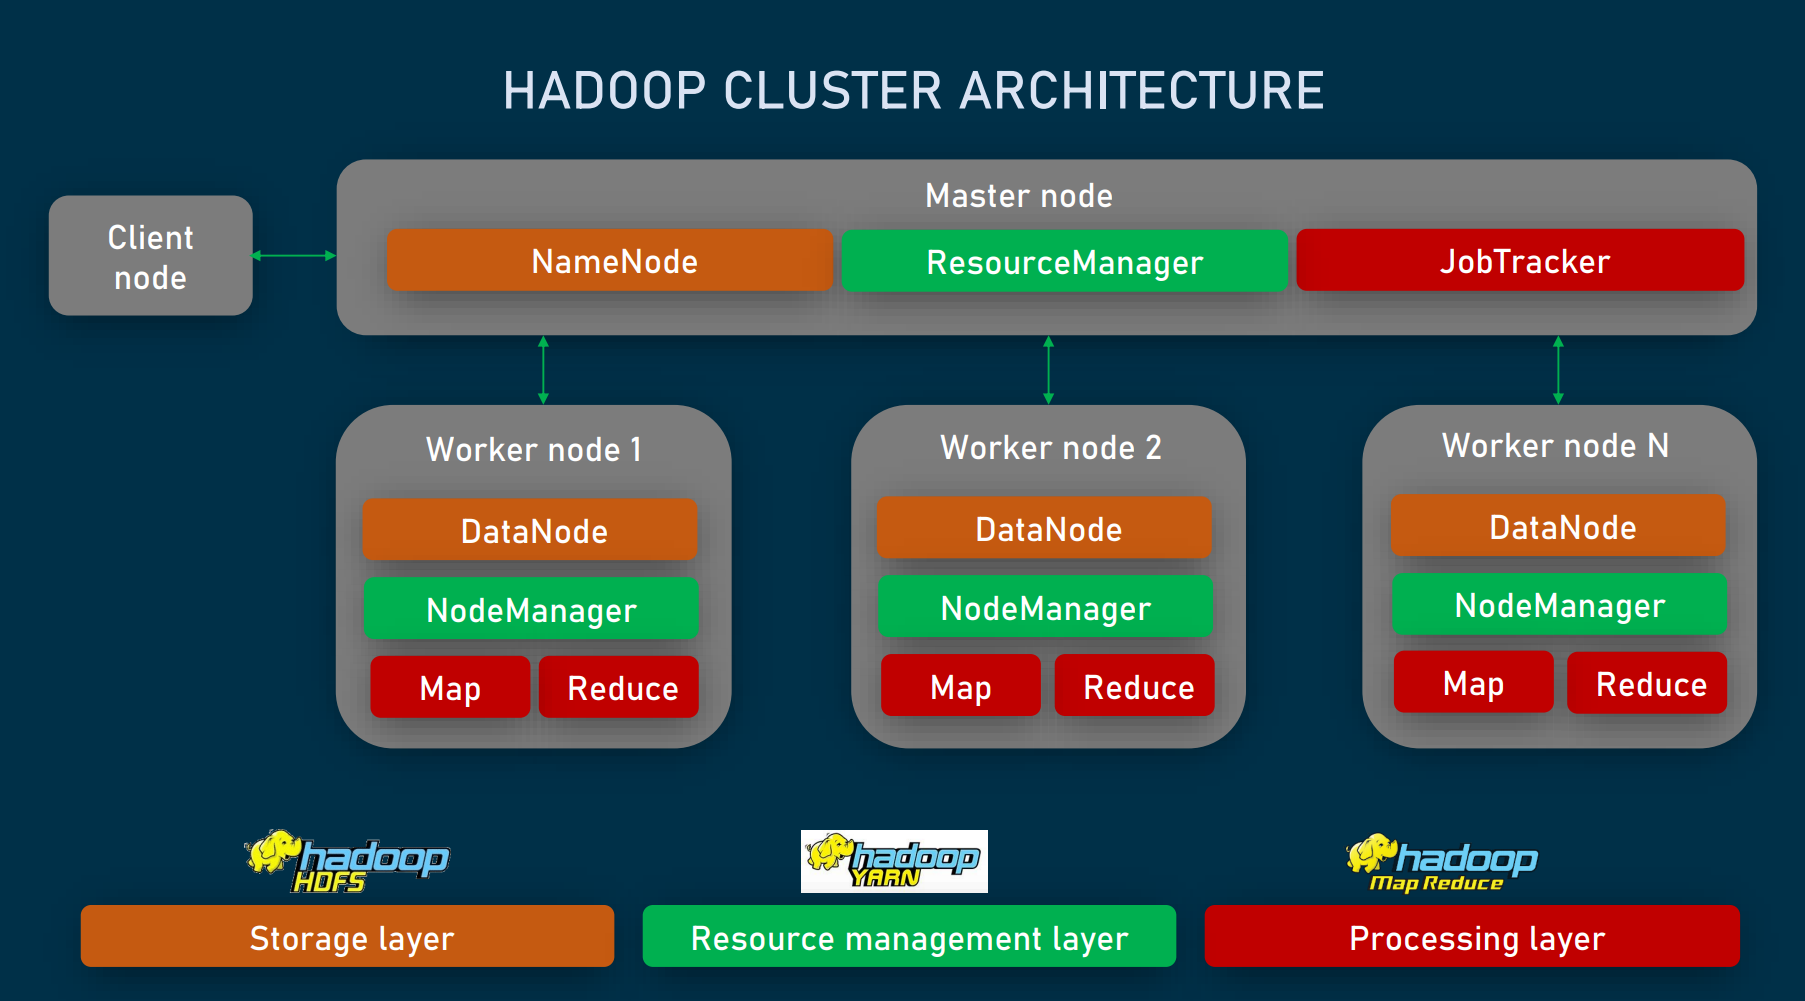
\includegraphics[width=\linewidth]{fig/hadoop_cluster.png}
    \caption{Apache Hadoop Architecture}
    \label{fig:architecture}
\end{figure}


\subsection{Experimental setup}
For this project we decided to use two different experimental setups. The primary setup contain total number of 4 nodes including one main Node and 3 data Node. The main node is named "group2" and words has been name "datanode" plus the consequent worker node order number (e.g., datanode1). All nodes had similar resources setup configuration as you can see in figure 2, there is 200~GB of HDD, 4~GB of RAM and two virtual CPU. Linux Ubuntu Forcal version 20.4 has been installed on all nodes as the operating system and Hadoop and Spark are each individually installed and configured on all nodes.
A secondary cluster configuration has also been considered which contains the same node configuration, but the total number of nodes has increased to 7 nodes including one main node and 5 worker nodes using the same naming policy.


The virtual network of the experimental setup is consisted of two networks. First one, public network and the second one group2 network which are connected together through a router.You can see the topology graph of the secondary cluster setup network on Figure~\ref{fig:topology}

\begin{figure}[t]
   \centering
   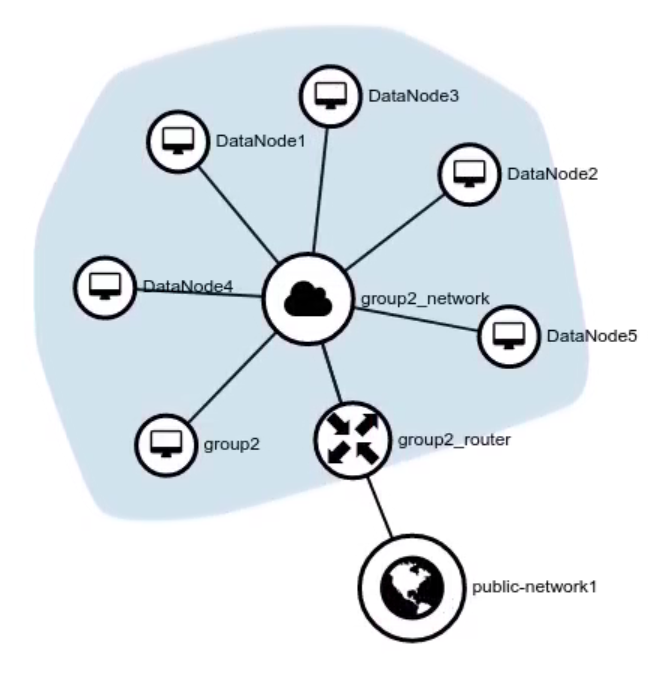
\includegraphics[width=\linewidth]{fig/NetworkTopology.png}
    \caption{Experimental Secondary Network Topology}
    \label{fig:topology}
\end{figure}

\section{Conclusion}
\label {sec:conclusion}
Here you need to summarize what you did and why this is
important. Do not take the abstract and put it in the past
tense. Remember, now the reader has (hopefully) read the
paper, so it is a very different situation from the abstract.
Try to highlight important results and say the things you really
want to get across such as high-level statements (e.g.,
we believe that .... is the right approach to .... Even though
we only considered LAN, the .... technique should be applicable
....) You can also formulate next steps if you want.
Be brief.

\section{Citation}
\label{sec:citation}
It is important that you correctly refer to sources. 

\begin{itemize}
\item If you describe background, according to some textbook, cite that textbook. \emph{See Example~\ref{def:consensus} below.}
\item If you make a claim about trends in industry or research, add citations to validate the claim. \emph{See Example~\ref{ex:trend} below.}
\item \textbf{Do not copy paste text from any source into your report without citation. It will be considered plagiarism.}
\item Always use the tilde character between the text and the cite command, e.g.:\begin{verbatim}
DBLP~\cite{dplg}
\end{verbatim}
The tilde inserts a space, but prevents line break between the text and citation.
\item For correct citations we recommend that you export bibtex entries from DBLP~\cite{dplg}. 
%@Hein: ACM produces crappy doi-urls for non ACM publications. I do believe that there are few papers that are part of the ACM-DL and not in DBLP.
But make sure to update the bibtex entries to adhere to the following rules.
\end{itemize}

Here are some rules to be followed for your bibliography:

\begin{itemize}
\item Make sure titles are correctly capitalized.

%You can export all nsdi citations from DBLP, accordingly this should not be a problem.
% \item Make sure abbreviations are consistent (e.g., is NSDI spelled out or
% not?) - using the @abbrev function in latex helps here.

\item Make sure there is enough info for a reader to find the document: authors
plus title isn't enough.

\item Don't blindly copy and paste ACM bibtex entries without fixing them:

- they list "New York, NY" as the address field, which means that all ACM
conferences look like they took place there; just delete this, or - better

- replace it with where the conference took place, which is much more
helpful to the reader than the publisher's address

- they have a truly weird idea about how to capitalize conference names;
just correct this (consistently)

* IEEE is equally bad, and uses a partially-inverted form of conference
names.

* Please actually review the bibliography before submitting your paper!
\end{itemize}

%@Leander: Move this to the Latex part:

And while you are at it, please:

\begin{itemize}
\item Add include{mathpmtc} in the main LaTeX file, so you don't have
math stuff in a different font than the main text. 
%We could simply add this to the template if not already done.

\item Always use the tilde character between the number and unit, e.g. 100~Mbps or 53~ms. 
The tilde inserts a space, but prevents line break between the number and unit.

\item Never put SI units in italics. 

\item Do differentiate between bits (b) and bytes (B), and between powers of 10~(MB) and 2~(MiB).

\item Avoid things like: "We refer the reader to [42]." That is, don't use citations as nouns.
\end{itemize}


\begin{example}
\label{def:consensus}
Consensus is a distributed programming abstraction that fulfills the following properties~\cite{aTextbook}:
\begin{description}
\item[Termination]
\item[Validity]
\item[Integrity]
\item[Agreement]
\end{description}
\end{example}

\noindent
\begin{example}
\label{ex:trend} Consensus systems build a fundamental part of todays cloud-computing infrastructure~\cite{spanner,chubby,zookeeper,zookeeperWeb}.
\end{example}




\section{Latex}
\label{sec:latex} 
This section contains some instructions and examples for using \LaTeX.

\subsection{You can add subsections}
You can use numbered subsections to structure your sections or $\backslash\texttt{paragraph}$ to separate paragraphs with a heading using only a few words, as used in Section~\ref{sec:introduction}.


\begin{enumerate}
	\item\label{item:1} This is an item in an enumeration.
    \begin{itemize}
    	\item This is an item of a unnumbered list. In this case, the lists are nested within each other.
    \end{itemize}
    \item\label{item:2} The second point in the enumerated list.
\end{enumerate}
%
I can refer to the element of the enumeration above as Point~\ref{item:1}.
If you refer to numbered items,~e.g. items from a list or figures or sections, always capitalize the name. 
For example, this is Section~\ref{sec:latex}.

\subsection{Figures}
You can include figures. You can include files, as done in Figure~\ref{fig:example}. 
Avoid including jpeg, gif or bmp files since these do not scale nicely. Again Figure~\ref{fig:example} is an example for that.

\begin{figure}[t]
   \centering
   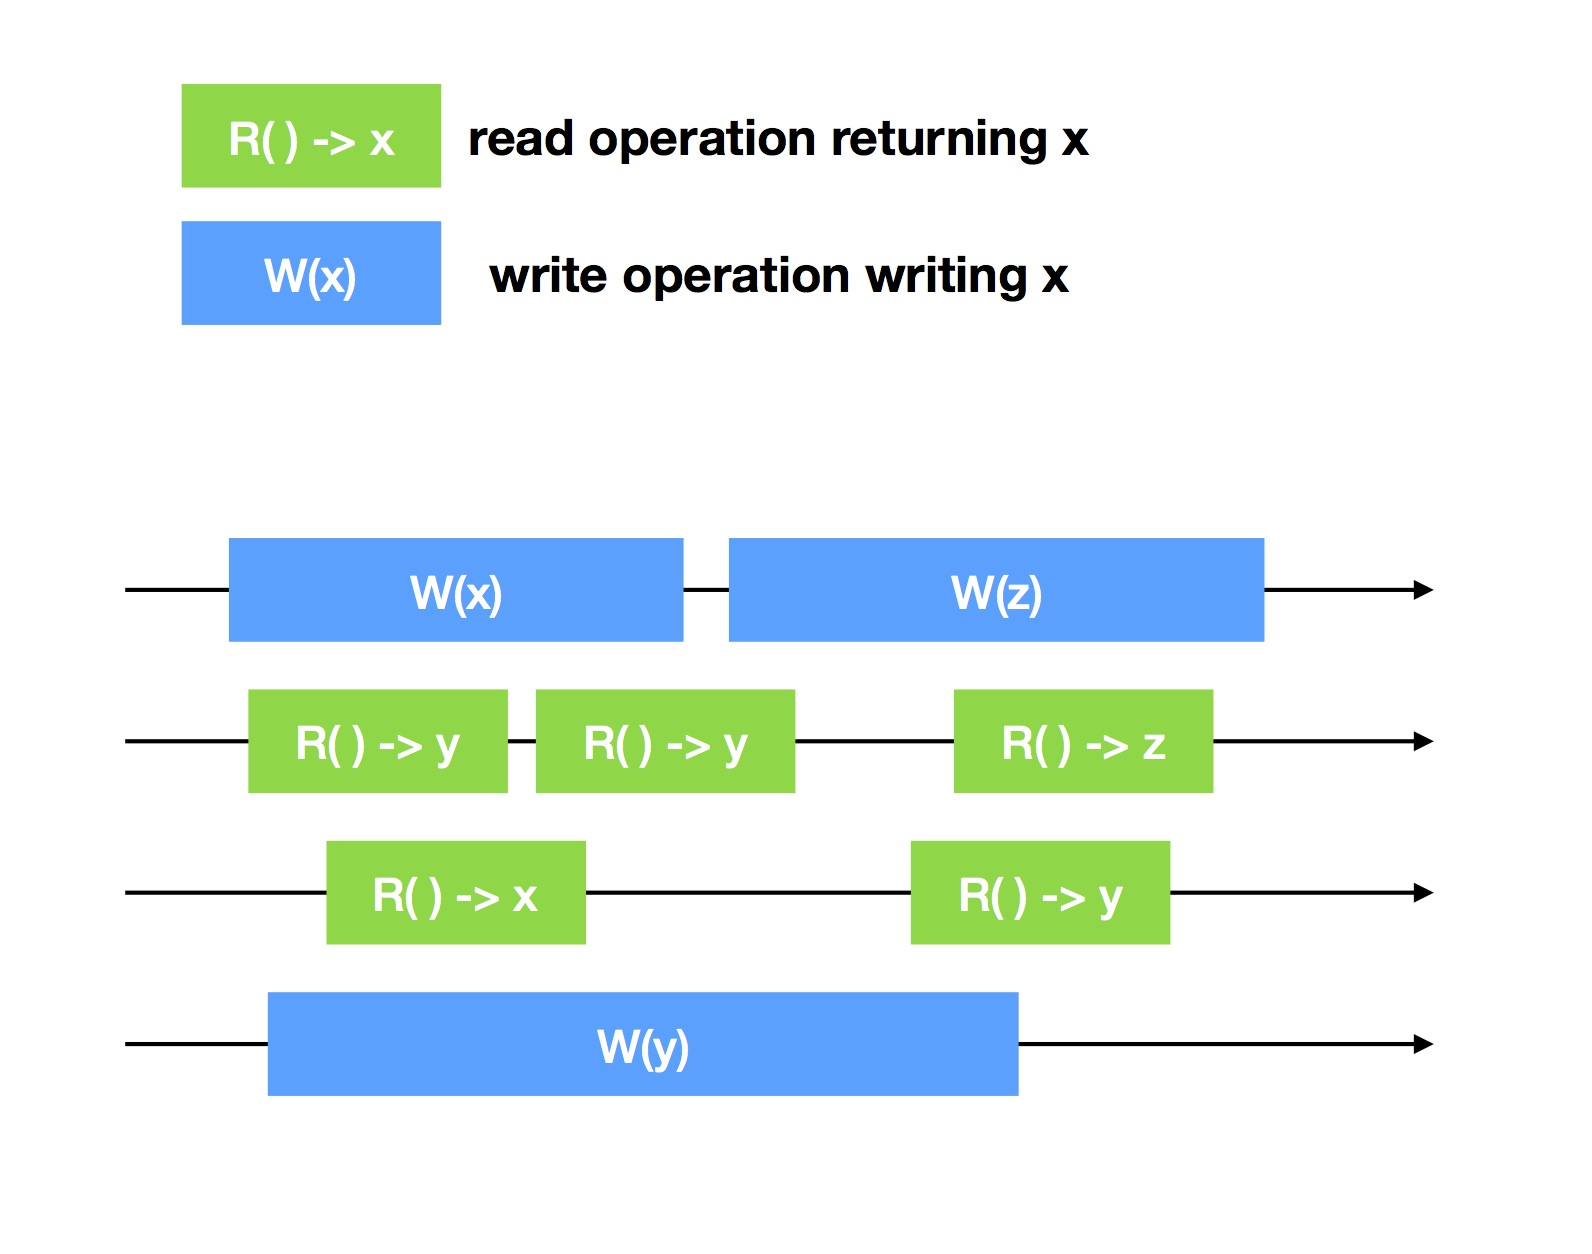
\includegraphics[width=\linewidth]{fig/RegisterOperations}
    \caption{Figure taken from~\cite{lecture}}
    \label{fig:example}
\end{figure}

You can create graphs from your experiment-data using \texttt{pgfplots}.
See the example in \texttt{tex/evaluation.tex} and documentation \url{http://pgfplots.sourceforge.net/pgfplots.pdf}.

\subsection{Other tips}
\begin{itemize}

\item Always use the tilde character between the number and unit, e.g. 100~Mbps or 53~ms. The tilde inserts a space, but prevents line break between the number and unit.

\item Never put SI units in italics. 

\item Do differentiate between bits (b) and bytes (B), and between powers of 10~(MB) and 2~(MiB).

\item Avoid things like: "We refer the reader to [42]." That is, don't use citations as nouns.
\end{itemize}

For further instructions on how to add \textbf{Tables, Algorithms, Theorems see acmguide.pdf}.


\section{Further Reading}
\label{sec:further}
Here are some other useful resources: (make these into references instead of links?)
\begin{itemize}
\item The co-chairs of the Ninth SOSP prepared some recommendations and valuable lessons in a paper titled \textit{How (and How Not) to Write a Good Systems Paper} \url{https://www.usenix.org/legacy/publications/library/proceedings/dsl97/good_paper.html}
\item \url{http://gramoli.redbellyblockchain.io/web/doc/talks/researchmethod.pdf}
\item \url{https://www.doc.ic.ac.uk/~prp/doc/talks/11-prp-paper_writing.pdf}
\item This template is inspired by a template from Markus P\"uschel~\cite{puschel}.

\end{itemize}

\bibliographystyle{ACM-Reference-Format}
\bibliography{sample-bibliography}

\end{document}
